\section{Instrumentation}

There are two main challenges on tracing processes’ progress with binary instrumentation ways in production systems. One is the performance issue. Even a lightweight static binary instrumentation usually pulls down execution time in several to several tens percentage, making speculative executions pyrrhic.  The other one is about exactness accuracy. The Ideal progress tracing is uniform with the real execution, which means that it can predict how much the task has been done and how long will it still last? Taking downloading a file for example, if the downloading progress bar shows a 50\% completion after 1 minute, it is clear about that half of the task has been done and it may still last about another 1 minute with a not too bad network. But for tasks running on the server nodes of cluster, heterogeneity between nodes, contentions for computing resources, imbalances in work-partitioning, all these restrictions prevent a reasonable prediction.

We primarily concern about the performance of tracing in N2O instrumenter, then overcome the second dilemma with N2O speculator requiring no accurate prediction, discussed in the next section.

With lots of case study, we refine two simple rules of binaries’ runtime behaviors. Functions in a binary can be placed in different level of an abstract syntax tree (AST). Functions in same level are often called with frequencies at similar order of magnitude in a range of executions, and the minority of functions in the top of call stack consume the majority of execution time, obviously a Pareto principle (80/20 principle). Table \ref{table:inst-stats} shows a sampling case with the ImageMagick dynamic link library. There are 1060 functions in the library and only 33 functions called more than 10000 times in about 100 millions functions hits of the sampling.

 \begin{table}[h]
\caption{statistics of samples of ImageMagick}
\label{table:inst-stats}
\begin{center}
\begin{tabular}{r|r|l}
\hline
Hits & Functions & Example \\
\hline
above 10e7 & 6 & CopyMagickMemory \\
10e6 - 10e7 & 16 & GetCacheNexus \\
10e5 - 10e6 & 2 & LocaleCompare \\
10e4 - 10e5 & 9 & GetNexus \\
10e3 - 10e4 & 10 & AddValueToSplayTree \\
10e2 - 10e3 & 17 & FormatMagickStringList \\
10e1 - 10e2 & 78 & NewSplayTree \\
10e0 - 10e1 & 922 & GaussianBlurImage \\
\hline
\end{tabular}
\end{center}
Note: only an example function name shows in the table.
\end{table}

As we know, the entry points and exit points of functions and basic blocks are common instrument points. For the progress tracing purpose, a naive idea is an instrument with all functions and basic blocks, even each cpu instruction. Unfortunately, the overhead is proportional to the hit rates. So with a little more coarse-grained instrumentation, skipping the minority of functions will reduce the majority of the overhead of instrumentation. Targeting extremely little overhead, we proposed a sampling based instrument approach. This goal has been achieved as the evaluation shown.

\section{Sampling}

The sampler is designed to instrument each function’s entry with a code snippet that records each function call and maintains the sampling data.The sampling data is saved in a key-value pattern: function name, call times. With varieties of executions, different level functions in the AST can be distinguished by the statistics results of the sampling data. The instrumenter first load the sampling data and a threshold T. Then it inserts a code snippet at entries of each function, but skipping those having a larger call times than threshold T. With the sampler directions, the instrumenter can instrument the binaries in an appropriate granularity. The instrumented binary is written as a file at last. 

We develop this instrument tool in a static instrumentation way based on DynIsnt library. Generally, there are three code snippets for the sampler: the initial one for creating some data structures for sampling, the final one for writing back the sampling data to a file, and the common used one for record a function call. For the instrumenter, the initial one for opening a file, the final one for closing a file, and the common used one just for increasing one to the number of tracepoints then writing it to the file. All the code snippets are carefully assembled with DynIsnt API and manipulated with the original binary. For the purpose of excellent performance, the instrumenter completes the file operations using the low level system call in the tmp directory, which is mounted as a RAM file system in Linux. It means that commonly several memory operations overhead is introduced into each function entry.

\section{Speculation}
For speculative executions, the first thing for N2O to do is finding the outliers. With the trace log returned by the instrumented processes, N2O use a Kmeans Clustering algorithm, which is commonly used in statistics analysis and data mining, to hunt the outliers. With outliers detected, N2O performs speculative executions, which needs interactive with job scheduler. 

\begin{figure}
\centering
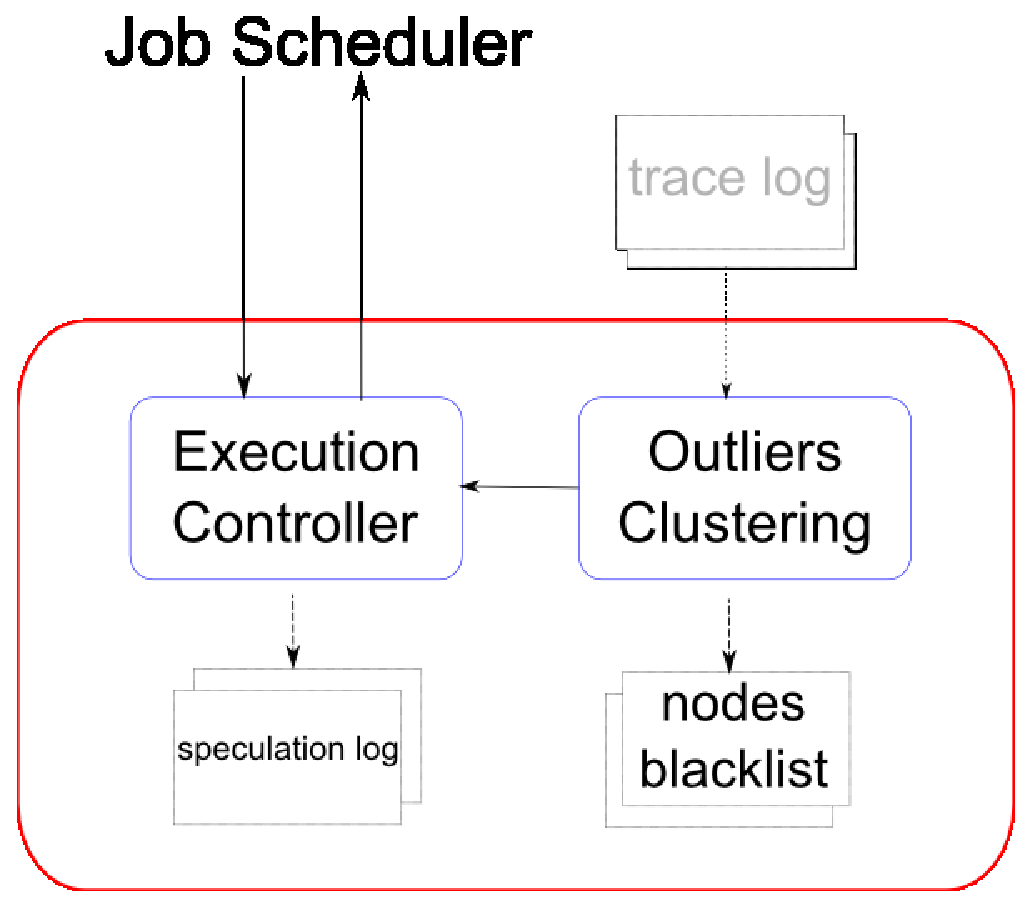
\includegraphics[width=0.9\columnwidth]{figures/speculator.eps}
\caption{Speculator Design}
\label{figure:speculator}
\end{figure}

As shown in Figure 2, two main components, Outliers Clustering and Execution Controller are corresponding to finding outliers and mitigate outliers by speculation. There are several assumptions for the speculator. Outliers is the minority in the massive parallel processes. The tasks is splitted with little imbalance. The server nodes of cluster becomes abnormal indeterminately and may return to normal after a while.

We novelly select two property of each executions to make outliers exposed, the number of tracepoints have been met TPN and the increment of tracepoints TPI in an interval. Figure 3 shows a possible example of two executions of the same binary at runtime, ideally they should draw the same line, but execution B is actually slower than execution A. It is similar to the results in the evaluation with N2O’s instrumenter. 

\begin{figure}
\centering
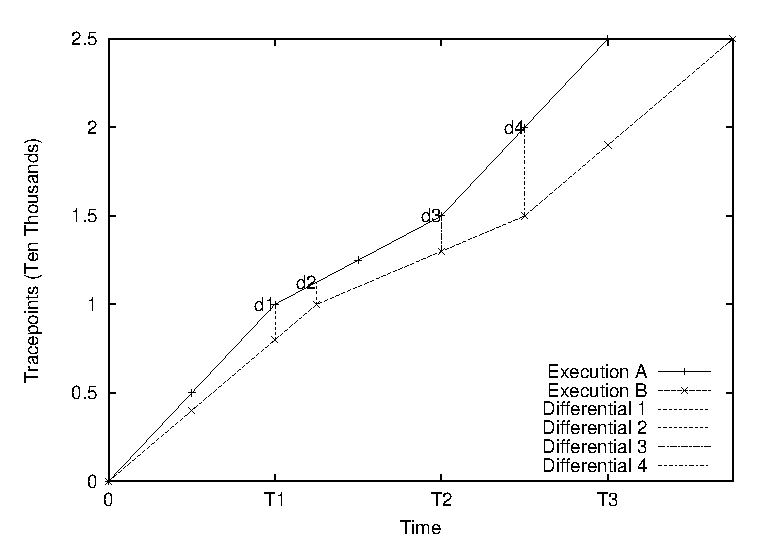
\includegraphics[width=0.9\columnwidth]{figures/executions_example.eps}
\caption{Executions Example}
\label{figure:executionsexample}
\end{figure}

A naive idea for exposing outliers is generating two clustering using a one-degree Kmeans Clustering algorithm, and if the coefficient of variation of the two clusterings’ means is larger than a threshold T, the clustering of executions with a less mean than the other one  will be seen as outliers.

But the number of tracepoints is not increased uniformly. We have proposed this dilemma at the binary instrumentation section. Four differential of two executions’ tracepoints has been marked as d1, d2, d3, d4 at four different time point. Although execution B is always 0.8x slower than execution A, the differential is not increased along the whole timeline. An obvious case is d1 > d2, this may lead to our naive approach mistaken execution B when clustering outliers. Another type of mistake is d3 < d4, execution B may just a little slower than execution A, but seen as an outlier in the naive approach. So there is no fixed threshold is appropriate for detection outliers with the naive idea.

To eliminate  the mistake caused by false positive and false negative, A improved approach has been come up with. We adjustment the threshold T multiplied by normalized mean of TPI of all executions. As one of the assumptions is outliers is minority, the mean of TPI of all executions is similar to the majority. This dynamic threshold can adaptive to the unstable increase of tracepoints perfectly.

The speculative execution algorithm for a job is straightforward with a few of heuristics improvement driven by several rules of thumb. These empirical rules are reasonable and verified in testing. The first rule is giving worst guy of outliers more speculation priority. As speculation is not completely free, it is obviously advisable speculation. Making sure of the split task and merge task not executing on irregular nodes is another important rule because of the impossible of exposing outlier with single task. On the other hand, the split and merge phases are always in the critical path of a job. The last one is speculation as soon as possible without irregular nodes. As the goal of speculation is early completion of job, speculation earlier and faster means better opportunity. The pseudo code of speculation algorithm is show in Fig. \ref{fig-spec-algo} :

 \begin{figure}
\textbf{Speculation Algorithm}
\begin{enumerate}[(1)]
\setlength{\itemsep}{-\itemsep}
\item update job info.
\item Loop with the following steps.
\begin{enumerate}[]
\setlength{\itemsep}{-\itemsep}
\item \textbf{Outliers Clustering}: First update the trace info, then make a Kmeans Clustering with the trace data. If CV > Threshold
\item \textbf{Speculation}: Sort outliers with speculative priority. For each outlier, if speculation is better, then executing on another node not in the blacklist.
\item Sleep several seconds and update job info. if the job has finished, break the loop and return.
\end{enumerate}
\end{enumerate}
\caption{Pseudocode of the speculation algorithm.}
\label{fig-spec-algo}
\end{figure}

We provide an execution controller implementation with ProActive Scheduler which can be interacted with  a control script. It invokes the outliers clustering module to establish outliers detection with updated trace data. Then maintaining a blacklist of nodes, each node in the blacklist has a penalty value. For outliers, generating a urgency job with only the speculative task and submitting in a speculation priority order. The constraints: no speculation on irregular nodes, can be achieved with a selection script and a claim of nodes selection in the job descriptor. The default speculation interval is 1 seconds, means that the interactive with the job scheduler is moderate. And each update of trace information has a little communication traffic, only an integer indicated the number of  tracepoints transmitted. This lightweight implementation is acceptable to the job scheduler and the impact of performance can be ignore.
